\documentclass[acmsmall,review,screen]{acmart}

%% TODO during camera-ready
%% copyright
\setcopyright{acmcopyright}
\copyrightyear{2024}
\acmYear{2024}
\acmDOI{XXXXXXX.XXXXXXX}

%% conference information
\acmConference[PLDI'24]{Make sure to enter the correct conference title from
your rights confirmation emai}{June 03--05, 2018}{Woodstock, NY}
\acmPrice{15.00}
\acmISBN{978-1-4503-XXXX-X/18/06}

%% macros with packages
% load packages
\usepackage{float}
\usepackage{amsmath,amsfonts}
\usepackage{algpseudocode}
\usepackage[ruled, vlined,linesnumbered]{algorithm2e}
\usepackage{graphicx}
\usepackage{textcomp}
\usepackage{xcolor}
\usepackage{soul}
\usepackage{listings}
\usepackage{caption}
\usepackage{subcaption}
\usepackage{multirow}
\usepackage{booktabs}
\usepackage{makecell}
\usepackage{galois}
\usepackage{mathpartir}
\usepackage{bussproofs}
\usepackage{mathtools}
\usepackage{colortbl}
\usepackage{hhline}
\usepackage{stmaryrd}
\usepackage{microtype}
\usepackage{hyperref}
\usepackage{balance}
\usepackage{adjustbox}
\usepackage{tikz}
\usepackage{csquotes}
\usepackage{url}
\usepackage{amstext} % for \text macro
\usepackage{array}   % for \newcolumntype macro

% box
\newcommand{\cfbox}[2]{%
  \colorlet{currentcolor}{.}%
  {\color{#1}%
  \fbox{\color{currentcolor}#2}}%
}
\newcommand{\lcolorbox}[2]{\adjustbox{padding=0ex 1ex 1ex 1ex, bgcolor=#1}{#2}}
\newcommand{\rcolorbox}[2]{\adjustbox{padding=1ex 1ex 0ex 1ex, bgcolor=#1}{#2}}

% table rules
\newcolumntype{?}{!{\vrule width 1pt}}
\newcommand*{\belowrulesepcolor}[1]{%
  \noalign{%
    \kern-\belowrulesep
    \begingroup
      \color{#1}%
      \hrule height\belowrulesep
    \endgroup
  }%
}
\newcommand*{\aboverulesepcolor}[1]{%
  \noalign{%
    \begingroup
      \color{#1}%
      \hrule height\aboverulesep
    \endgroup
    \kern-\aboverulesep
  }%
}

% colors
\definecolor{gainsboro}{rgb}{0.86, 0.86, 0.86}
\definecolor{dkgreen}{rgb}{0, 0.5, 0}
\definecolor{lightred}{rgb}{0.93, 0.57 0.52}
\definecolor{esnt}{rgb}{0.20, 0.20, 0.20}
\definecolor{esparam}{rgb}{0.16, 0.63, 0.59}
\definecolor{esalg}{rgb}{0.12, 0.42, 0.65}
\definecolor{esvar}{rgb}{0.16, 0.63, 0.59}
\definecolor{gray1}{rgb}{0.95, 0.95, 0.95}
\definecolor{gray2}{rgb}{0.85, 0.85, 0.85}
\definecolor{gray3}{rgb}{0.75, 0.75, 0.75}

\newcolumntype{L}{>{$}l<{$}} % math-mode version of "l" column type
\newcommand{\llb}{\llbracket}
\newcommand{\rrb}{\rrbracket}

% basic
\newcommand*{\sphinxDeclareColorOption}[2]{%
   \definecolor{#1}#2%
}%
\sphinxDeclareColorOption{InnerLinkColor}{{rgb}{0.208,0.374,0.486}}
\newcommand{\inblue}[1]{{\color{InnerLinkColor}{#1}}}
%\newcommand{\inblue}[1]{{\color{blue}{#1}}}
\newcommand{\inred}[1]{{\color{red}{#1}}}
\newcommand{\x}[1]{\inred{#1}}
\newcommand{\y}[1]{\textbf{\inred{#1}}}
\newcommand{\todo}{\inred{TODO}}
%\newcommand{\powerset}{\mathcal{P}}
\newcommand{\tif}{\text{if} \; }
\newcommand{\telse}{\text{otherwise}}
\newcommand{\tst}{{\; \text{s.t.} \; }}

% Our tool name
\newcommand{\name}[1]{\textsf{#1}\xspace}
\newcommand{\ssf}[1]{\ensuremath{\mathsf{#1}}\xspace}
\newcommand{\sbf}[1]{\textbf{\small #1}\xspace}
\newcommand{\stt}[1]{\texttt{\small #1}\xspace}
\newcommand{\dsl}{\name{Wasm-DSL}}
\newcommand{\dl}{\name{DL}}
\newcommand{\al}{\name{AL}}
\newcommand{\spectec}{\name{\$SRC}}
\newcommand{\dslname}{SpecTec\xspace}
\newcommand{\ires}{\ssf{IR_{\mathsf{ES}}}}

% codes
\newcommand{\code}[1]{\text{\lstinline[style=JS]!#1!}} 
\newcommand{\scode}[1]{\texttt{\scriptsize #1}} 
\newcommand{\bcode}[1]{\texttt{\small #1}}
\newcommand{\ircode}[1]{\text{\lstinline[style=ires]!#1!}}

\newcommand{\kwsyn}{\bcode{syntax}}
\newcommand{\kwret}{\bcode{return}}

\newcommand{\kwalg}{\bcode{algorithm}}
\newcommand{\kweq}{\coloneqq}
\newcommand{\kwdef}{\bcode{def}}
\newcommand{\kwif}{\bcode{if}}
\newcommand{\kwreturn}{\bcode{return}}
\newcommand{\kweither}{\bcode{either}}
\newcommand{\kwenter}{\bcode{enter}}
\newcommand{\kwassert}{\bcode{assert}}
\newcommand{\kwpush}{\bcode{push}}
\newcommand{\kwpop}{\bcode{pop}}
\newcommand{\kwpopall}{\bcode{popall}}
\newcommand{\kwlet}{\bcode{let}}
\newcommand{\kwtrap}{\bcode{trap}}
\newcommand{\kwnop}{\bcode{nop}}
\newcommand{\kwexecute}{\bcode{execute}}
\newcommand{\kwexecuteseq}{\bcode{executeseq}}
\newcommand{\kwperform}{\bcode{perform}}
\newcommand{\kwexit}{\bcode{exit}}
\newcommand{\kwref}{\bcode{ref}}
\newcommand{\kwreplace}{\bcode{replace}}
\newcommand{\kwiscaseof}{\bcode{iscaseof}}
\newcommand{\kwisdefined}{\bcode{isdefined}}
\newcommand{\kwisvalid}{\bcode{isvalid}}
%\newcommand{\kwwasmc}{\bcode{wasmc}}
%\newcommand{\kw}{\bcode{}}
\newcommand{\kwnot}{\bcode{not}}
\newcommand{\kwequ}{\bcode{=}}
\newcommand{\kwrl}{\bcode{(}}
\newcommand{\kwrr}{\bcode{)}}
\newcommand{\kwcl}{\bcode{\{}}
\newcommand{\kwcr}{\bcode{\}}}
\newcommand{\kwsl}{\bcode{[}}
\newcommand{\kwsr}{\bcode{]}}
\newcommand{\kwass}{\bcode{:=}}
\newcommand{\kwext}{\bcode{:+}}
\newcommand{\kwcat}{\bcode{++}}

\newcommand{\unop}{\ensuremath{\otimes}}
\newcommand{\binop}{\ensuremath{\oplus}}

% Basic
\DeclareMathAlphabet{\mathpzc}{T1}{pzc}{m}{it}
\newcommand{\powerset}[1]{\mathcal{P}(#1)}
\newcommand{\abs}[1]{\widehat{#1}}
\newcommand{\finmap}{{\xrightarrow[]{\text{fin}}}}
\newcommand{\mapstos}{\;\dot{\mapsto}\;}
\newcommand{\Dom}{\name{Dom}}
\DeclarePairedDelimiter{\norm}{\lvert}{\rvert} 

% JavaScript
\newcommand{\js}{\name{js}}

% Getters
\newcommand{\getfunc}{\name{func}}
\newcommand{\getinst}{\name{inst}}
\newcommand{\getnext}{\name{next}}
\newcommand{\getcaller}{\name{caller}}
\newcommand{\getlab}{\name{label}}

% Values
\newcommand{\valset}{\mathbb{V}}
\newcommand{\val}{v}
\newcommand{\pvalset}{\valset^\name{p}}
\newcommand{\pval}{\val^\name{p}}
\newcommand{\boolset}{\valset_\name{bool}}
\newcommand{\bool}{b}
\newcommand{\true}{\code{\#t}}
\newcommand{\false}{\code{\#f}}
\newcommand{\intset}{\valset_\name{int}}
\newcommand{\strset}{\valset_\name{str}}

% JavaScript ASTs
\newcommand{\treeset}{\mathbb{T}}
\newcommand{\tree}{t}
\newcommand{\trees}{\overline{t}}
\newcommand{\nodeset}{\Phi}
\newcommand{\node}{\phi}
\newcommand{\subtree}{\lhd}
\newcommand{\getsubs}{\name{subs}}
\newcommand{\treetop}{\code{\#}}
\newcommand{\ty}{\tau}
\newcommand{\eval}{\code{eval}}

% DL Syntax
\newcommand{\defnset}{\mathfrak{D}}
\newcommand{\defn}{d}
\newcommand{\infrset}{\mathcal{R}}
\newcommand{\infr}{r}
\newcommand{\funcset}{\mathcal{F}}
\newcommand{\func}{f}

% AL Syntax
\newcommand{\progset}{\mathfrak{P}}
\newcommand{\prog}{p}
\newcommand{\algset}{\mathcal{A}}
\newcommand{\alg}{a}
\newcommand{\instset}{\mathcal{I}}
\newcommand{\inst}{i}
\newcommand{\exprset}{\mathcal{E}}
\newcommand{\expr}{e}
\newcommand{\condset}{\mathcal{C}}
\newcommand{\cond}{c}
\newcommand{\numset}{\mathcal{N}}
\newcommand{\num}{n}
\newcommand{\qualset}{\mathcal{Q}}
\newcommand{\qual}{q}
\newcommand{\wasmcset}{\mathcal{W}}
\newcommand{\wasmc}{w}
\newcommand{\cnstrset}{\mathcal{K}}
\newcommand{\cnstr}{k}

% Variables
\newcommand{\varset}{\mathcal{X}}
\newcommand{\varx}{x}
\newcommand{\varf}{f}
\newcommand{\vart}{t}
\newcommand{\varp}{p}

% Field Mappings
\newcommand{\fmapset}{\mathbb{M}}
\newcommand{\fmap}{m}
\newcommand{\jsfmapset}{\fmapset_\js}
\newcommand{\jsfmap}{\fmap_\js}

% Transition Relations
\newcommand{\trans}[1]{\leadsto_{#1}}

\newcommand{\hide}[1]{}
\newcommand{\unify}{\ensuremath{\mathcal{U}}\xspace}
\newcommand{\dltoil}{\ensuremath{\mathcal{T}}\xspace}


%% start document
\begin{document}

%% title information
\title{
SpecTec: Bridging the Gap between Declarative and Algorithmic Semantics
}

\author{Anonymous Author(s)}

%% authors
%
% \author{Dongjun Youn}
% \email{f52985@kaist.ac.kr}
% \orcid{0000-0002-5766-2035}
% \affiliation{%
%   \institution{KAIST}
%   \city{Daejeon}
%   \country{South Korea}
% }
%
% \author{Wonho Shin}
% \email{???@kaist.ac.kr}
% \orcid{????-????-???-????}
% \affiliation{%
%   \institution{KAIST}
%   \city{Daejeon}
%   \country{South Korea}
% }
% \author{Jaehyun Lee}
% \email{???@kaist.ac.kr}
% \orcid{????-????-????-????}
% \affiliation{%
%   \institution{KAIST}
%   \city{Daejeon}
%   \country{South Korea}
% }
%
% \author{Sukyoung Ryu}
% \email{sryu.cs@kaist.ac.kr}
% \orcid{0000-0002-0019-9772}
% \affiliation{%
%   \institution{KAIST}
%   \city{Daejeon}
%   \country{South Korea}
% }

%% abstract
\begin{abstract}
WebAssembly (Wasm) is a versatile binary instruction format enabling
high-performance code execution across diverse environments. As Wasm gains
momentum with continuous feature enhancements, the specification of its
execution semantics becomes pivotal. Wasm-DSL has emrged as an innovative
approach to streamline the meticulous documentation process: Wasm-DSL is used
as front-end language to define semantics and the generation of both formal and
prose notations as back-ends is automated. While generating formal notations is
relatively straightforward, the challenge of generating accurate and consistent
prose notations arises due to the fundamental disparity between prose and
formal notations.

This paper presents Algorithmic Language (AL), an executable language designed
to resemble prose, automating the generation of precise prose descriptions. AL
is extracted from Wasm-DSL, and a comprehensive testing framework validates its
correctness.  This approach addresses the challenges posed by manual
specification composition and offers a transformative solution for enhancing
the accuracy and efficiency of programming language specifications.
\end{abstract}



%% TODO http://dl.acm.org/ccs.cfm during camera ready
% \begin{CCSXML}
% <ccs2012>
%  <concept>
%   <concept_id>10010520.10010553.10010562</concept_id>
%   <concept_desc>Computer systems organization~Embedded systems</concept_desc>
%   <concept_significance>500</concept_significance>
%  </concept>
%  <concept>
%   <concept_id>10010520.10010575.10010755</concept_id>
%   <concept_desc>Computer systems organization~Redundancy</concept_desc>
%   <concept_significance>300</concept_significance>
%  </concept>
%  <concept>
%   <concept_id>10010520.10010553.10010554</concept_id>
%   <concept_desc>Computer systems organization~Robotics</concept_desc>
%   <concept_significance>100</concept_significance>
%  </concept>
%  <concept>
%   <concept_id>10003033.10003083.10003095</concept_id>
%   <concept_desc>Networks~Network reliability</concept_desc>
%   <concept_significance>100</concept_significance>
%  </concept>
% </ccs2012>
% \end{CCSXML}
%
% \ccsdesc[500]{Computer systems organization~Embedded systems}
% \ccsdesc[300]{Computer systems organization~Redundancy}
% \ccsdesc{Computer systems organization~Robotics}
% \ccsdesc[100]{Networks~Network reliability}
\keywords{
  WebAssembly,
  language specification,
  executable prose,
  DSL,
}

\maketitle

%% body of the paper
\section{Introduction}\label{sec:intro}

WebAssembly, commonly referred to as Wasm, is a versatile and efficient binary
instruction format that enables high-performance execution of code across
diverse environments, from web browsers to edge devices. The design philosophy
of Wasm revolves around platform independence, security, and efficient
performance, resulting in a versatile technology that bridges the gap between
high-level programming languages and the web ecosystem. As the adoption of Wasm
gains momentum, a continuous stream of new features is incorporated, extending
the capabilities of the language.

At the heart of WebAssembly's functionality lies its execution semantics, which
define how WebAssembly programs operate. The behavior of a WebAssembly program
is defined in terms of an abstract machine that models the program's state.
This abstract machine encompasses a stack to record operand values and control
constructs, as well as an abstract store housing global state information. The
execution process unfolds by iteratively executing each instruction of the
WebAssembly program, one step at a time. Each step alters the internal state of
the abstract machine, with the precise effects being specified by reduction
rules within the operational semantics.

The official WebAssembly specification~\cite{wasmspec} meticulously documents
the execution semantics using the LaTeX framework, presenting them in two
complementary yet equivalent forms: prose and formal notation. Prose notation
provides a stepwise, algorithmic description of WebAssembly's execution
semantics, offering explicit guidance on the operations to be executed on
various parts of the program state and their sequential order. This prose
notation aims to provide a human-readable understanding of how WebAssembly
instructions operate.  In contrast, formal notation articulates these semantics
through mathematical, declarative rules. This formal representation closely
resembles the original operational semantics, comprising reduction rules that
correspond to each WebAssembly instruction. The dual representation serves to
cater to comprehension of both language implementers and designers, ensuring
clarity and correctness within the language specification.

\begin{figure}
  \centering
  \begin{subfigure}[b]{0.45\textwidth}
    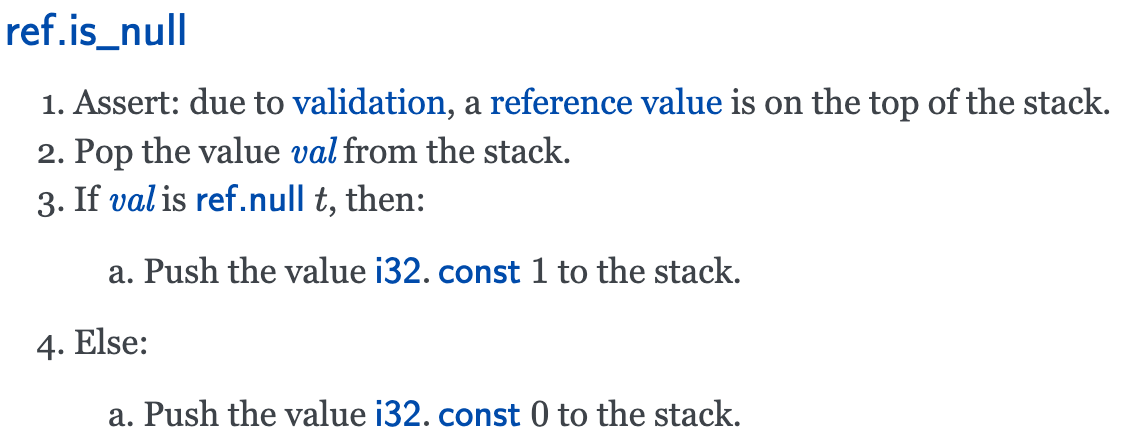
\includegraphics[width=\textwidth]{img/prosespec1}
    \caption{Prose notation}
    \label{fig:prosespec1}
  \end{subfigure}
  \hfill
  \begin{subfigure}[b]{0.45\textwidth}
    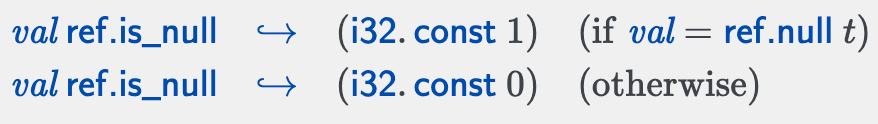
\includegraphics[width=\textwidth]{img/formalspec1}
    \caption{Formal notation}
    \label{fig:formalspec1}
  \end{subfigure}
  \begin{subfigure}[b]{0.45\textwidth}
    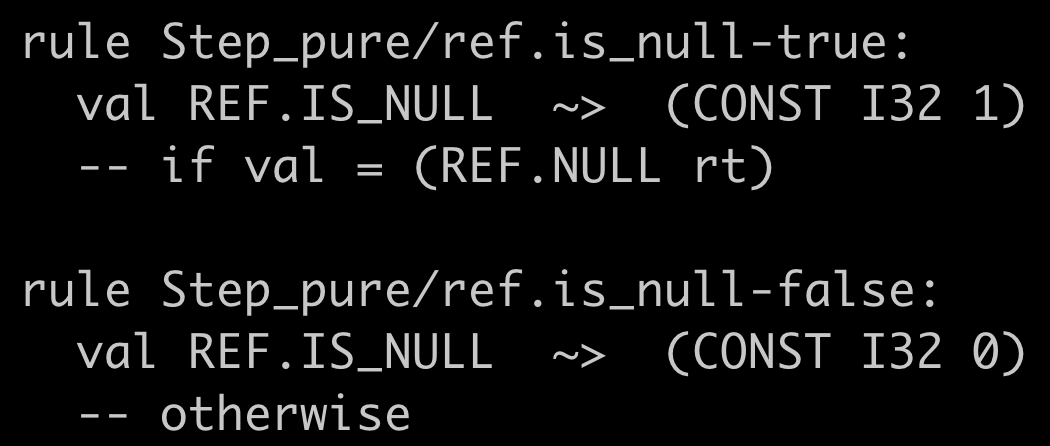
\includegraphics[width=\textwidth]{img/dsl1}
    \caption{DSL}
    \label{fig:dsl1}
  \end{subfigure}

  \caption{Semantics of `ref.is\_null`}
  \label{fig:spec1}
\end{figure}

In Figure~\ref{fig:spec1}, we present an illustration of how the specification
defines the execution semantics of the `ref.is\_null` WebAssembly instruction.
This instruction evaluates whether a given WebAssembly value is null. In
Figure~\ref{fig:prosespec1}, we specify its behavior using prose notation. The
description begins by asserting the existence of a value with a type of
`reference` at the top of the stack in line 1. Subsequently, in line 2, the
value is removed from the stack.  Depending on whether the removed value is
`ref.null t` or not, either the integer value 1 or 0 is pushed onto the stack
in lines 3-a or 4-a, respectively. In Figure~\ref{fig:formalspec1}, we provide
the operational semantics using formal notation. The reduction rule specifies
the shape of the stack before and after executing one step, potentially with
side conditions indicating when this reduction should occur. For instance, the
stack `val ref.is\_null` should reduce to (i32.const 1) only if `val` equals
`ref.null t`, and otherwise, it should reduce to (i32.const 0).

%Creating and maintaining this meticulous specification holds paramount
%significance as it forms the foundation for consistent and reliable behavior
%among WebAssembly programs across different implementations. This is crucial
%because developers, implementers, and tool creators need a comprehensive
%understanding of these semantics. This understanding is essential for building
%WebAssembly implementations that are not only robust but also optimized for
%efficiency, with the specification playing a pivotal role in facilitating this
%understanding. The ongoing evolution and growing adoption of WebAssembly
%further emphasize the heightened importance of precision and clarity within
%this documentation. As the WebAssembly ecosystem continues to develop and
%establish its presence, the accuracy and clarity of the specification become
%even more critical to ensure smooth integration and dependable execution.

The challenge of manually crafting and maintaining precise specifications is
particularly daunting due to the intricate nature of the documentation process.
Compounded by the utilization of the complex LaTeX typesetting system, the
manual authorship of these specifications becomes a laborious and error-prone
endeavor. It demands meticulous attention to detail for accurate
representation, making it susceptible to various errors, typos, or
inconsistency within specification. A case in point is the incorporation of 5
proposals for new features into Wasm 2.0. A substantial number of new
instructions, including a staggering 80 SIMD instructions, were added,
necessitating the manual composition of both formal and prose specifications
for each instruction. Moreover, the specifications of several existing
instructions underwent modifications. In the midst of this process, several
errors found its way into the specification of new or modified insturctions,
one of which took two years to be rectified. This example, exemplified by the
expansion to Wasm 2.0, underscores the challenges posed by manually crafting and
maintaining the specification, demanding a labor-intensive process and
entailing the risk of errors. Given Wasm's planned extensions beyond 3.0,
driven by over 25 proposals, addressing this challenge becomes increasingly
critical.

In response to the challenges of crafting precise specifications manually, the
Wasm community has introduced a promising solution in the form of $\dsl$
(WebAssembly Domain Specific Language). It is a domain-specific language
tailored to describing the standard of WebAssembly, including its execution
semantics. $\dsl$ serves as the single source of truth for the Wasm semantics.
Once the operation semantics of WebAssembly is articulated using this
specialized language, numerous other 'representations' of the semantics can be
automatically generated, including interpreters, test suites, mechanized
proofs, and notably, the specification document.  By translating $\dsl$ as
front-end into LaTex for both formal and prose specification as back-ends,
documenting the specification becomes a more streamlined process, potentially
reducing the burden of manual specification writing.  Moreover, this systematic
translation provides much higher confidence in the trustworthiness of the
generated specification compared to a manually generated one.

The key advantage of $\dsl$ lies in its ability to offer a clear, visually
aligned representation of the operational semantics of WebAssembly that is easy
to read and write. Figure~\ref{fig:dsl1} illustrates the semantics of
`ref.is\_null`, described using $\dsl$. Just like the operational semantics,
each reduction rule contains the left-hand side and right-hand side notating
the stack of the abstract machine before and after the reduction, and premises
denoting the condition for that reduction to happen.

Generating a formal notation specification from $\dsl$ is relatively
straightforward, thanks to this design. Since both $\dsl$ and formal
specifications adopt a declarative approach based on mathematical reduction
rules, the translation from $\dsl$ to formal notation can be achieved through a
single, linear scan of the $\dsl$. This one-to-one correspondence minimizes the
risk of generating a specification that deviates from the intended execution
semantics outlined in $\dsl$. Even in cases where discrepancies arise, they can
be readily identified and rectified.

Generating prose notation specification, however, presents a distinct and
intricate challenge. In contrast to $\dsl$, prose notation entails an
algorithmic, step-by-step description of execution semantics. The translation
between these two styles is not straightforward, as it necessitates the mapping
of declarative statements to algorithmic prose while ensuring consistency with
the formal specification.

\begin{figure}
  \centering
  \begin{subfigure}[b]{0.45\textwidth}
    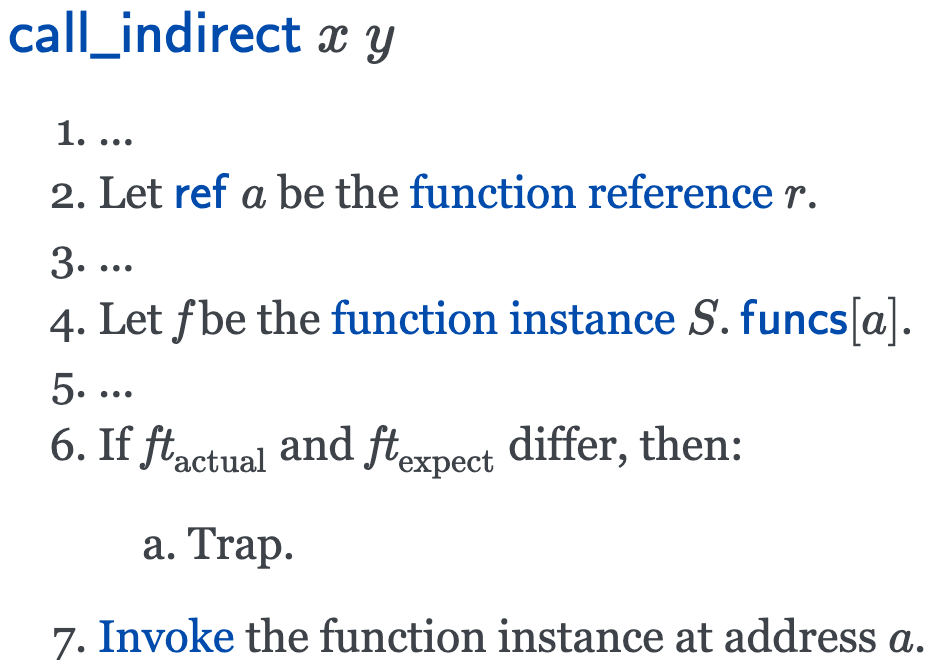
\includegraphics[width=\textwidth]{img/prosespec2}
    \caption{Prose notation}
    \label{fig:prosespec2}
  \end{subfigure}
  \hfill
  \begin{subfigure}[b]{0.45\textwidth}
    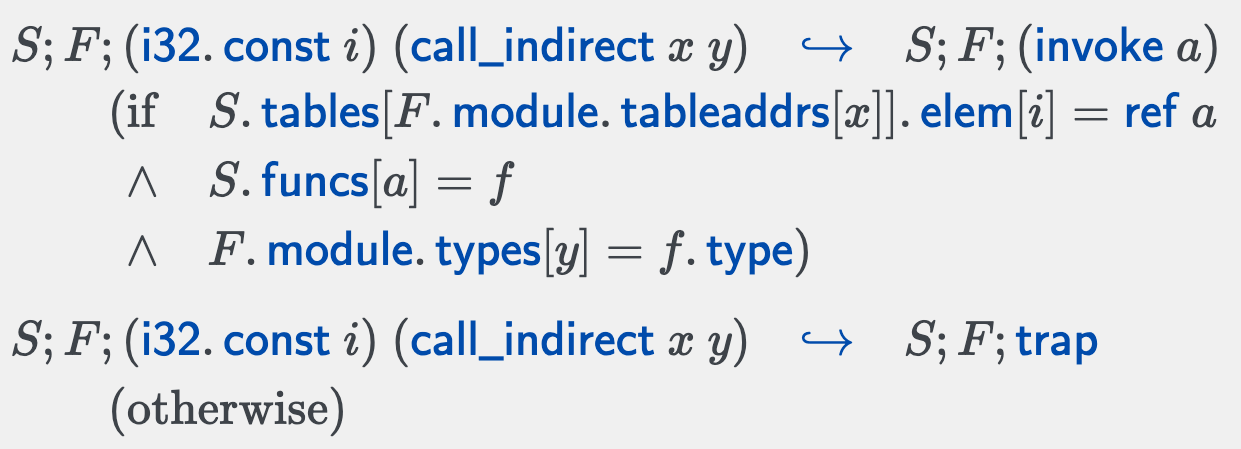
\includegraphics[width=\textwidth]{img/formalspec2}
    \caption{Formal notation}
    \label{fig:formalspec2}
  \end{subfigure}

  \caption{Semantics of `call\_indirect`}
  \label{fig:spec2}
\end{figure}

Figure~\ref{fig:spec2} illustrates one of these challenges, depicting the
manually-written specifications of the Wasm `indirect\_call` instruction. In
the formal specification (Figure~\ref{fig:formalspec2}), three premises are
presented, each comprising a simple equality. These premises are translated
into three instructions on line 2, 4, and 6 in the prose specification
(Figure~\ref{fig:prosespec2}), respectively. Notably, despite their identical
format of simple equality, some of these equalities are intended to establish a
new variable, while others are designed to serve as conditions. Consequently,
the first two are translated into the `Let` statement, as seen in lines 2 and 4,
while the last premise is transformed into the `If` statement in line 6. Adding
to the complexity, the three premises in the formal specification could be
arranged in any order, but the translated statements must adhere to a specific
fixed order due to interdependencies. This problem of inferring the role and
order of the premises, which we refer to as "animation," has been shown to be
NP-hard.

Furthermore, the inherent disparity between prose and formal notations poses a
challenge in ensuring that the generated prose accurately reflects the intended
behavior of the formal semantics. As an illustration, the prose specification
in Figure~\ref{fig:prosespec2} introduces temporary variables, such as
ft\_actual or ft\_expect, which were absent in the formal specifications
presented in Figure~\ref{fig:formalspec2}. This divergence complicates manual
verification of consistency since one must meticulously track such deviations.
Given that the process of prose generation is notably susceptible to errors due
to its intricate translation nature, the pursuit of a methodology to
systematically verify its alignment with the formal notation stands as a
substantial research endeavor.

In response to these challenges, we propose a novel solution: Algorithmic
Language ($\al$), an executable language that closely resembles the structure
and style of prose notation. Our approach seeks to automate and enhance the
process of generating prose descriptions from the formal semantics described in
$\dsl$. We achieve this in two pivotal steps. First, we establish an automated
pipeline for the translation of $\dsl$ into $\al$. Subsequently, we generate
prose descriptions by stringifying the translated $\al$. We also identify the
challenges encountered during the process including the animation problem
previously mentioned, and suggest the effective, lightweight solutions for
them. Furthermore, to underscore the correctness and reliability of the
generated prose, we have developed an interpreter for $\al$ which enables
automatic and rigorous testing of the behavior described by the translated
$\al$ against the official WebAssembly test suite. Our results confirm the
consistency and accuracy of our methodology, boasting a 100\% pass rate across
official WebAssembly tests, thereby validating the fidelity of the generated
prose descriptions.

In summary, this paper offers the following key contributions:

\begin{itemize}
\item We provide a formal definition of the syntax and semantics of
Algorithmic Language ($\al$), an executable language designed to resemble prose
specification.
\item We present an automated method for generating prose specification from
the execution semantics of Wasm described in $\dsl$, and provide the solutions for
the identified challenges during the process.
\item We establish the correctness and reliability of our automatically
generated prose descriptions by subjecting them to comprehensive testing
against the official Wasm test suite.
\end{itemize}

The subsequent sections of this paper will delve into the specifics of our
methodology, detailing the creation of $\al$, the translation process from
$\dsl$ into $\al$ and the identified challenges, the development of the $\al$
interpreter, and the comprehensive testing framework employed. Through this
exploration, we aim to not only address the challenges associated with prose
notation in Wasm, but also explore the potential of $\al$ as a transformative
tool for enhancing the accuracy and efficiency of programming language
specifications in general.

\section{AL}\label{sec:al}

This section explains about syntax and semantics of AL.
\footnote{Note that this is NOT a syntax and semantics of WebAssembly, but rather,
syntax and semantics of prose notation of WebAssembly Specification}

\subsection{syntax}

This section describes the syntax of AL.

\begin{minipage}{0.5\textwidth}
$$
\begin{array}{@{}lrrl@{}}
& \mathsf{p} &::=& {\mathsf{A}^\ast} \\
& \mathsf{A} &::=& \mathsf{algorithm}~\mathit{f}~({\mathit{e}^\ast})~\{{\mathsf{i}^\ast}\} \\
& \mathsf{i} &::=& \mathsf{if}~\mathit{c}~{\mathsf{i}^\ast}~{\mathsf{i}^\ast} \\ &&|&
\mathsf{either}~{\mathsf{i}^\ast}~{\mathsf{i}^\ast} \\ &&|&
\mathsf{assert}~\mathit{c} \\ &&|&
\mathsf{push}~\mathit{e} \\ &&|&
\mathsf{pop}~\mathit{e} \\ &&|&
\mathsf{popall}~\mathit{e}~\mathit{c} \\ &&|&
\mathsf{peek}~\mathit{e}~\mathit{c} \\ &&|&
\mathsf{let}~\mathit{e}~\mathit{e} \\ &&|&
\mathsf{call}~{\mathit{e}^?}~\mathit{f}~{\mathit{e}^\ast}~\{{({\mathit{x}^\ast} ; \mathit{iter})^\ast}\} \\ &&|&
\mathsf{trap} \\ &&|&
\mathsf{nop} \\ &&|&
\mathsf{return}~{\mathit{e}^?} \\ &&|&
\mathsf{execute}~\mathit{e} \\ &&|&
\mathsf{jumpin}~\mathit{e} \\ &&|&
\mathsf{jumpout} \\ &&|&
\mathsf{getfirst}~\mathit{e}~\mathit{c} \\ &&|&
\mathsf{replace}~\mathit{e}~\mathit{p}~\mathit{e} \\ &&|&
\mathsf{append}~\mathit{e}~\mathit{e} \\ &&|&
\mathsf{appendlist}~\mathit{e}~\mathit{e} \\
& \mathit{c} &::=& \sim\mathit{c} \\ &&|&
\mathit{c}(\wedge)\mathit{c} \\ &&|&
\mathit{e}(<)\mathit{e} \\ &&|&
!\mathit{e} \\ &&|&
\mathit{e}<:\mathit{s} \\ &&|&
\mathsf{valid}~\mathit{e} \\
\end{array}
$$
\end{minipage}
\begin{minipage}{0.5\textwidth}
$$
\begin{array}{@{}lrrl@{}}
& \mathit{e} &::=& \mathit{n} \\ &&|&
\mathit{s} \\ &&|&
\mathit{op}(\mathit{e^\ast}) \\ &&|&
\mathit{e}^\ast \\ &&|&
\mathit{e}^\mathit{e} \\ &&|&
\mathit{e}::\mathit{e} \\ &&|&
|\mathit{e}| \\ &&|&
\{{(\mathit{text} \rightarrow \mathit{e})^\ast}\} \\ &&|&
\mathit{e}[\mathit{p}] \\ &&|&
\mathit{e}[\mathit{p}^\ast:+=\mathit{e}] \\ &&|&
\mathit{e}[\mathit{p}^\ast:=\mathit{e}] \\ &&|&
\mathit{s}(\mathit{e}^\ast) \\ &&|&
\mathit{e}^? \\ &&|&
(\mathit{e},\mathit{e}) \\ &&|&
\mathit{x} \\ &&|&
\mathit{e}^{\{\mathit{x}^\ast\}~\mathit{iter}} \\
& \mathit{iter} &::=& \mathsf{?} \\ &&|&
\mathsf{\ast} \\ &&|&
\mathsf{+} \\ &&|&
{(\mathit{x}<)}^?~\mathit{e} \\
& \mathit{p} &::=& [\mathit{e}] \\ &&|&
[\mathit{e}:\mathit{e}] \\ &&|&
.\mathit{s} \\
\end{array}
$$
\end{minipage}

Metavariable
$\mathsf{p}$ ranges over a program,
$\mathsf{A}$ ranges over an algorithm,
$\mathsf{i}$ ranges over an instruction,
$\mathit{c}$ ranges over a condition,
$\mathit{e}$ ranges over an expression,
$\mathit{iter}$ ranges over an iter-expression,
$\mathit{p}$ ranges over a path,
$\mathit{n}$ ranges over an integer,
$\mathit{s}$ ranges over a string,
$\mathit{x}$ ranges over a variable name.
and
$\mathit{f}$ ranges over a function name.

An AL program $\mathsf{p}$ consists of algorithms $\mathsf{A}^\ast$.  An
algorithm $\mathsf{A}$ has its name $\mathit{f}$, parameters
${\mathit{e}^\ast}$, and its body instructions ${\mathit{i}^\ast}$.  There are
various types of instructions including familiar push/pop instructions. The
instructions are designed in a way that it resembles the prose statements
appearing in the official specification.  For example, the prose `2. Pop the
value val from the stack` in Fig~\ref{fig:prosespec1} corresponds to the following
instruction: $\mathsf{pop} \mathit{val}$. There are also various kinds of
conditions and expressions.
\subsection{semantics}

This section describes the semantics of AL. It is based on an abstract machine
that models the program state, which consists of a stack and a store. An
algorithm is a entry point of an execution. One can execute a algorithm of the
program by calling it.  When an algorithm is called, the body instructions of
the algorithm are interpreted sequentially.

Interpreting one instruction may alter the internal program state of the
abstract machine, and the exact effect of each instruction is described using
semantics rule.

Figure ???  illustrate the rules for interpreting each
kind of instruction.
\inred{TODO: Write semantics of AL instructions in more detail. REQUIRED: Actually finish formalizing the semantics of AL.}

Conditions are calculated into a
boolean value, and the expressions are evaluated into a value.

Figure ??? illustrate the rules for calculating each kind of condition in
big-step semantics. \inred{TODO: Explain semantics of AL conditions in more detail.}

Figure ??? illustrate the rules for evaluating each kind of expression in big-step
semantics. \inred{TODO: Write semantics of AL expressions in more detail.}

Note that both calculating conditions and evaluating expressions are pure and
do not have any side-effect on the program state.



\section{Translating Wasm-DSL into AL}\label{sec:translate}

In this section, we describe the translation process of Wasm-DSL into AL.

Wasm-DSL can express whole standard of the WebAssembly, including not only
execution semantics but also syntax and validation rules.
Since generating prose from execution semantics is the main goal of this paper,
we will only focus on how execution semantics of Wasm is expressed using Wasm-DSL, but not syntax or validation.

Two kinds of \textit{definitions} are needed to express the execution semantics of Wasm:
reduction rules and auxiliary helper functions.

\subsection{Notations}
Here, we formally define the notations for the reduction rules and the auxiliary helper functions.

A reduction rule $\ruleW \in \rulesW = \configsW \times \configsW \times \premsW^\ast$ is a triplet of a
configuration \textit{lhs}, a configuration \textit{rhs}, and a finite sequences of premises \textit{prem}*.

A configuration $\configW \in \configsW = E_\bot \times E$ is a tuple of an optional expression for state \textit{s},
and an expression for a finite sequence of Wasm instructions, \textit{winstrs}.

A premise $p \in \premsW = B \uplus \{otherwise\}$ is either a boolean expression, or a
single `otherwise` whose high-level interpretation is "negation of all previous premises".

\textbf{Example.} Recall the semantics of `ref.is\_null` in figure~\ref{fig:dsl1}.
The first rule will be parsed into the following reduction rule:
\[r_1=(\bot, [val, \text{REF.IS\_NULL}]), (\bot, [\text{CONST I32 1}]), [val = (\text{REF.NULL rt})]\]
The second rule will be parsed into the following:
\[r_2=(\bot, [val, \text{REF.IS\_NULL}]), (\bot, [\text{CONST I32 0}]), [otherwise]\]
Note that both of lhs and rhs for both rules are omitting the state expression,
and thus we notate it by using $\bot$.

The high-level interpretation of a reduction rule $r = (lhs, rhs, prem*)$ should be straightforward:
when the current configuration of the program matches \textit{lhs} and all \textit{prem}s are
evaluated to be true, then alter the program configuration into \textit{rhs}.

A helper function $\helperW \in \helpersW = NAME \times E^\ast \times E \times \premsW^\ast$ is a quadruple of
the name, parameters \textit{params}, a return expressions \textit{ret}, and a finite sequences of premises \textit{prem}*.

\textbf{Example.} \inred{TODO: Give a example of a helper function}

\subsection{Transformation}
In this section, we describe the transformation of \dsl~into \al.

\begin{figure}
  \centering
  \begin{subfigure}[b]{0.9\textwidth}
    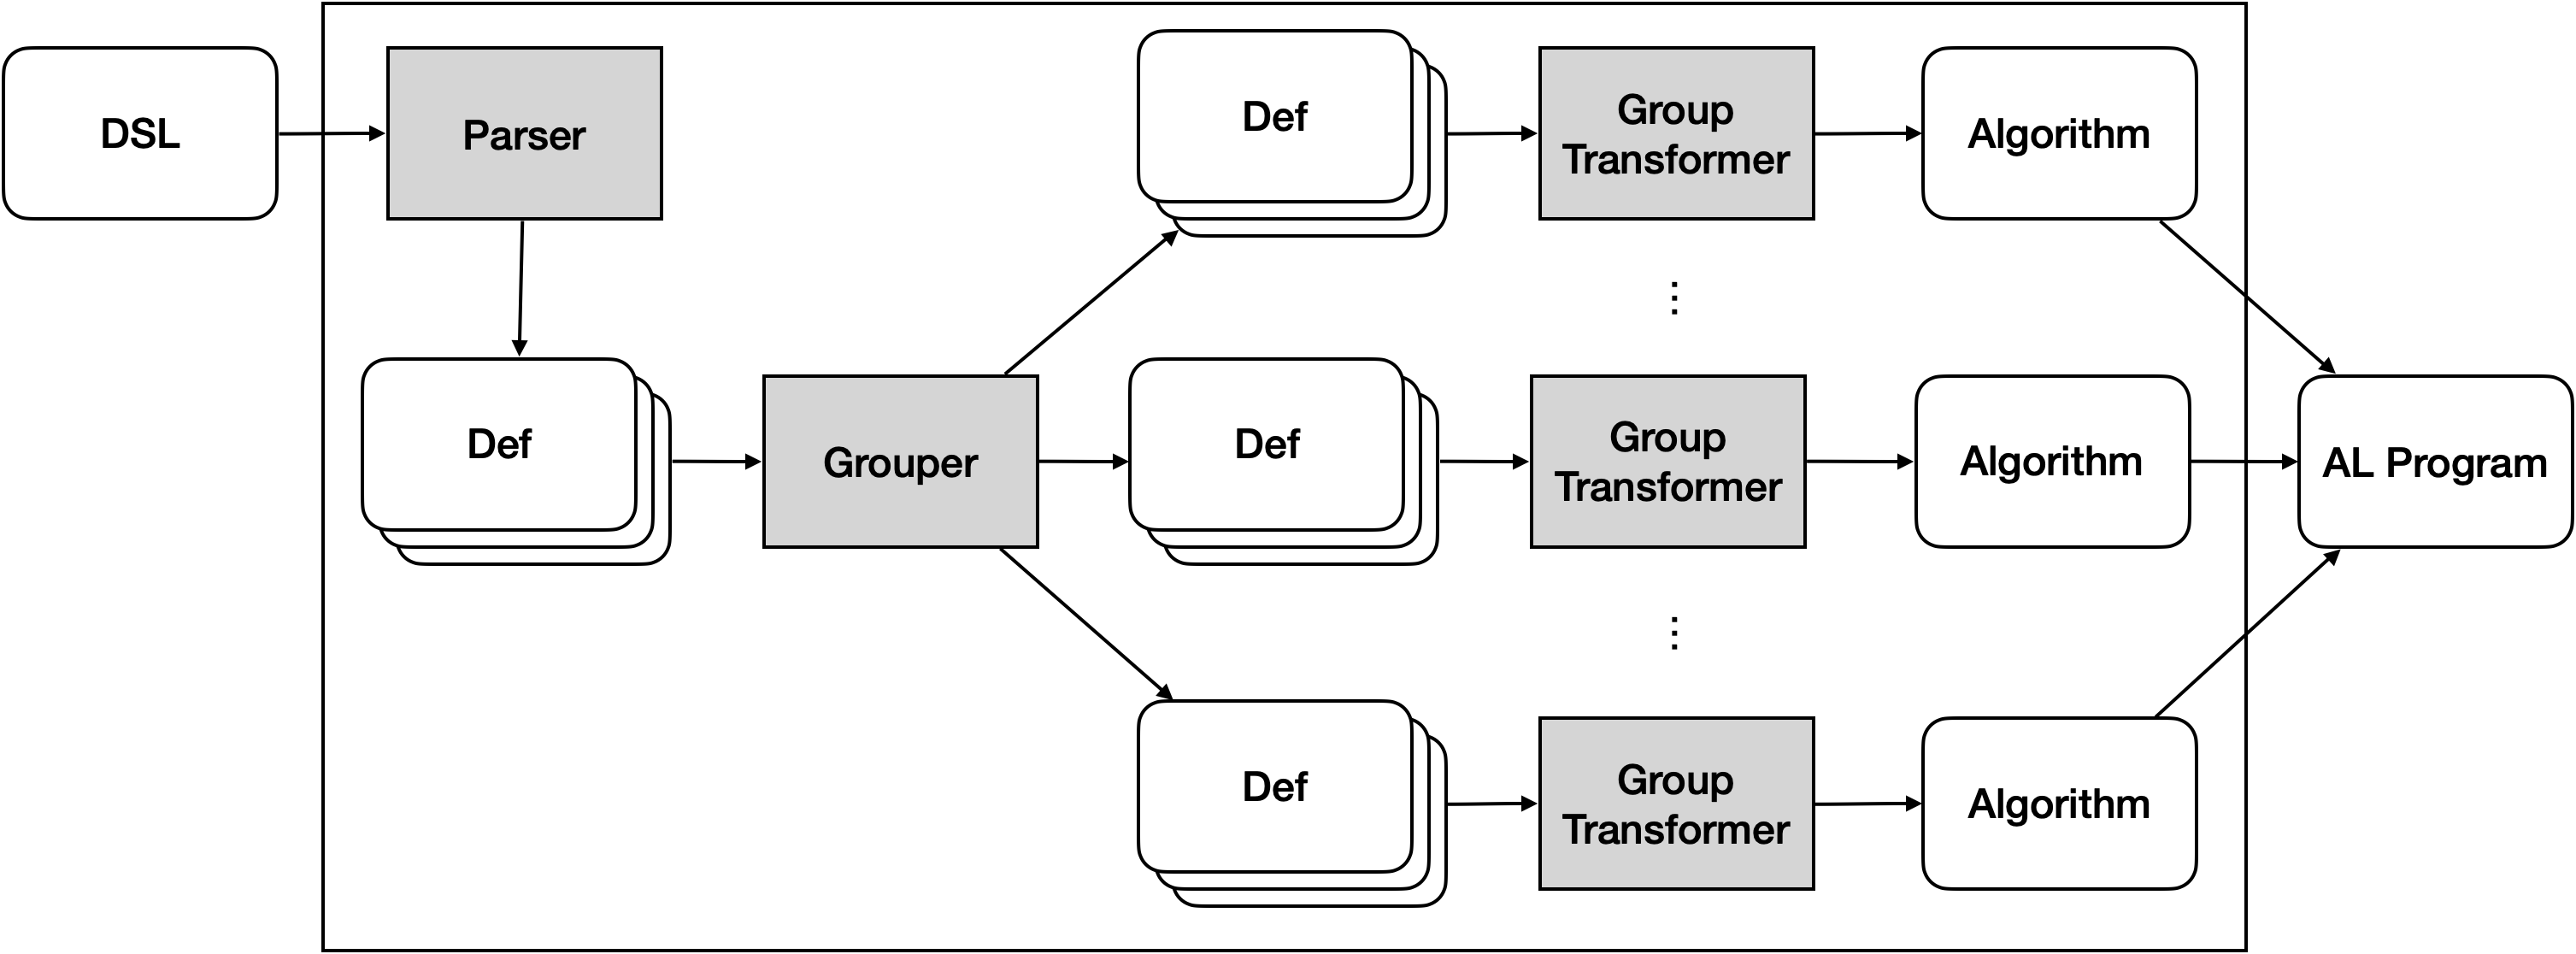
\includegraphics[width=\textwidth]{img/trans1}
    \caption{Overview}
    \label{fig:overview}
  \end{subfigure}
  \hfill
  \begin{subfigure}[b]{0.9\textwidth}
    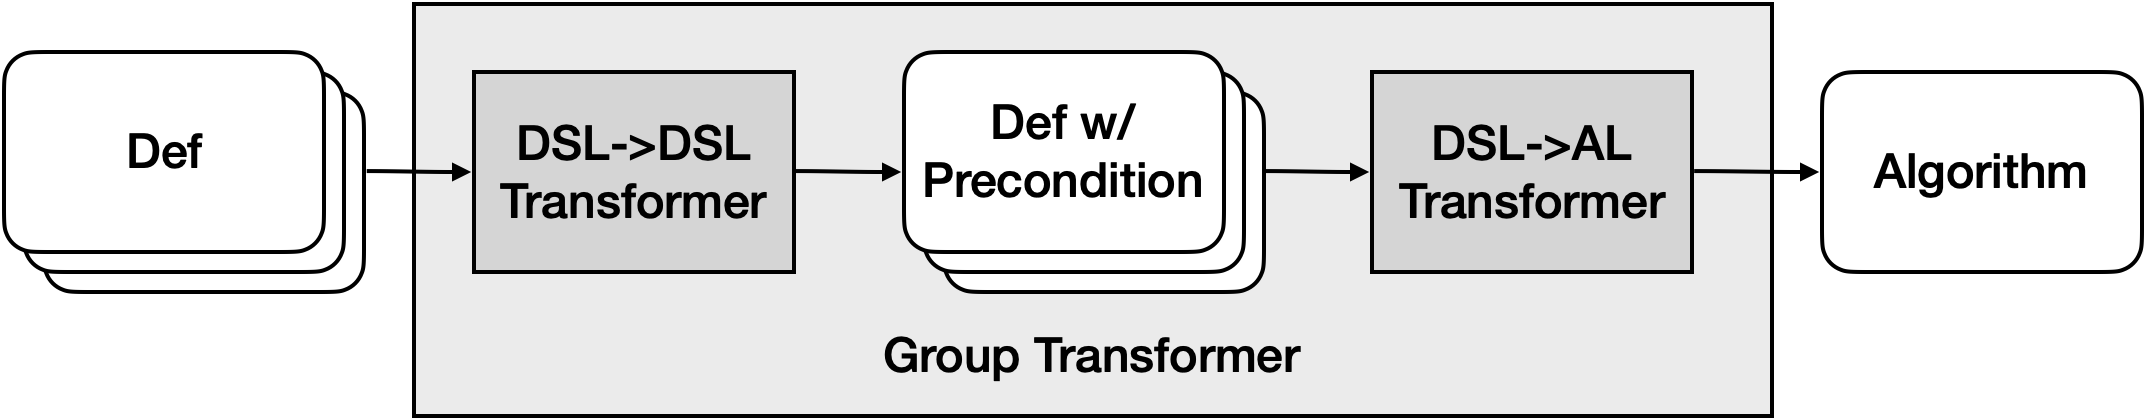
\includegraphics[width=\textwidth]{img/trans2}
    \caption{Group transformer}
    \label{fig:grouptrans}
  \end{subfigure}
  \caption{DSL->AL transformation}
  \label{fig:trans}
\end{figure}


Figure~\ref{fig:overview} shows the whole system of transforming DSL into an \al~program.
The input of the system is the \dsl~document,
and the output of the system is a single \al~program $\mathsf{p}$.
The input undergoes the following process of transformation.
First, the input DSL is parsed into a set of definitions: either a reduction rule or a
helper function. Then, the definitions are grouped. Reduction rules are grouped based on
their target Wasm instruction, and helper functions are grouped based on their names.
As a result, multiple groups are formed. Each group is transformed into a single algorithm,
$\mathsf{A}$. The transformed algorithms are collected into a single AL program, which is the
final output of this transformation system. This AL then can be stringified into a
prose notation specification document, or can be coupled with the AL interpreter to form a Wasm interpreter.

Figure~\ref{fig:grouptrans} shows the detail of group transformer, a component of the Figure~\ref{fig:overview}.
The input is either a group of reduction rules \textit{r}, or a group of helper functions \textit{h}.
The output is a single algorithm.
Due to the fundamental difference between mathematical rules and algorithm,
directly transforming into an algorithm is a non-trivial task.
Therefore, the process is divided into two steps: first pre-process DSL so that
it becomes more suitable for transformation, and then transform it into an algorithm.
As a first step, a group of definitions are first transformed into a different but equivalent group of definitions,
so that the new transformed group of definitions satisfies certain \textit{preconditions}.
The preconditions are there to help generate AL algorithms with more ease.
If the input group already satisfies the precondition, then this transformation will keep the input intact.
Secondly, Then new group of definition is transformed into AL.
How the AL is generated slightly differ based on whether the group is a reduction rule group or a helper function
group, but they are both based on the following fundamental approach.
% Should I explain AL -> AL?

\subsubsection{DSL->DSL transformation}

There are two major steps for transforming DSL into DSL: 1. LHS/Parameter unification and
2. animation.

\textbf{1. LHS / Parameter Unification}

Unification is a step that makes all LHS (for reduction rule) or parameters
(for helper functions) identical within the group.
This precondtion already holds for most cases, with a few exceptions.
The most notable example is the `br` instruction.
Here are two simplified reduction rules for the `br` instruction
\[
r_1 = (..., [... \text{(BR 0)} ...]),  (..., ...), []
\]
\[
r_2 = (..., [... \text{(BR l+1)} ...]),  (..., ...), []
\]
The intention here is that `br l` instruction should be applied with different rule,
depending on whether l is 0 or not.
Note that the both rules do not have any premise. The condition check is implicitly assumed to be
done when matching the current configuration with LHS.

The following is the result of unification:
\[
r_1' = (..., [... \text{(BR t)} ...]),  (..., ...), [t = 0]
\]
\[
r_2' = (..., [... \text{(BR t)} ...]),  (..., ...), [t = l + 1]
\]
The temporary variable t is introduced for both rules, replacing 0 of the first rule and
l+1 of the second rule. In order to denote what the temporary variable originally was
in each rules, new premise is added, denoting t equals 0 in the first rule, and l+1 in the second rule.

\inred{
  TODO: Explain algorithm/method of animation: walking two AST's simultaneously.
}


\textbf{2. Animation}

There are two problems that makes it challenging to transform premises into AL.
First, if a given premise is an equality expression, then it may work as either a simple condition or
a binding of a new variable, and this should be inferred. More formally, it is required to
correctly find out where each free variable is getting bound. Second, the order
of premises can be permutated in an arbitrary order. This is problematic for
generating algorithm, since the exact order of steps are crucial in the algorithm.

Animation is a step that addresses these two challanges. Its goal is to infer
the bound variables and the order of each premise.
After animation, each premise is tagged with what variables it is binding
such that every variables are bound exactly once, and premises are ordered in a way that
all of unbound variables in each premise is already bound by the previous premises.

We have discovered that this solving the animation problem is in fact NP-hard.
We prove it by reduction from a known NP-hard problem, an exact cover problem.

Theorem: Animation problem is NP-hard.

Proof: \inred{TODO}

This theorem implies that there is no trivial method for solving this problem.
One obvious solution to this kind of problem is probably using a SMT solver such as Z3, since
this problem is fundamentally a constraint problem.
However, using such a heavy tool seems to be a bit over-engineering for this rather small input.
Instead, we decided to use a simple yet effective approach.
We reduce the problem into a exact cover problem\footnote{Note that the direction is opposite with
the proof}, and then adopt the well-known effective algorithm to solve exact cover problem,
the Knuth algorithm[?].

\inred{
  TODO: Explain reduction to exact cover and Knuth algorithm to solve it
}.


\subsubsection{DSL->AL transformation}

In this section, we explain the transformation of DSL with preconditions into an AL algorithm.

----------------

Algorithm 1.

Input: A group of reduction rules r* = (lhs, rhs, prems)*

Output: An algorithm $\mathsf{A}$

1. lhs <- r*[0].lhs

2. instrs <- lhs\_to\_instr(lhs)

3. For r in r*:

--a. prems = r.prems

--b. rhs = r.rhs

--c. instr\_prems <- prems\_to\_instr(prems)

--d. instr\_rhs <- rhs\_to\_instr(rhs)

--e. instrs <- instrs ++ merge(instr\_prems, instr\_rhs)

4. (name, params) <- extract\_name\_and\_params(lhs)

5. Return ($\mathsf{algorithm}$ name (params) {instrs})

----------------

\inred{TODO: Pretty print algorithm 1}


After the group is transformed, the next step is to
change each group into an algorithm. Algorithm 1 depicts the pseudocode of the transformation
of group of reduction rules into an algorithm.
First, the lhs of this reduction rule group is extracted on line 1, and is transformed into
an AL instructions on line 2. Since it is guaranteed that every lhs of reduction rule are
identical, any lhs from any rules of the group can be used. This transformed list of instructions
will be used as an initial list, and will grow iteratively by the loop on line 3.
Premises and rhs are extracted for each reduction rule on line a and b, and then transformed into
instructions on lines c and d. These two lists of instructions are merged to form a single
list of instructions, and then accumulatively appended to the intial instruction list.
Finally, the name and parameter of this algorithm should be extracted from the target instruction of the reduction rule,
which itself is obtained from any lhs of the rule on line 4. At last, the name, parameters, and
AL instructions will be packed and returned as the final algorithm.

\inred{
  TODO: Explain lhs\_to\_instr, prems\_to\_instr, rhs\_to\_instr, merge, extract\_name\_and\_params
}

\section{Evaluation}\label{sec:eval}

This section explains about evaluation.

\section{Related Work}\label{sec:related}

This section explains about related works.

Related about language-describing frameworks
-> Ott / K-Framework / etc.
-> ESMeta

Related about turning animation
-> Original animation paper, maybe Datalog or relational DB should be investigated.

\section{Conclusion}\label{sec:conclusion}
To address the challenge of extracting prose specification of Wasm from DSL, we
introduced Algorithmic Language (AL), an executable language closely mirroring
the structure and style of prose notation. AL serves as an intermediary step in
the automated generation of precise prose descriptions from Wasm-DSL. We
established an automated pipeline for extracting AL from Wasm-DSL and validated
the correctness of these descriptions by developing an AL interpreter and
subjecting it to rigorous testing against the official WebAssembly test suite.
Our results showcased a 100\% pass rate, affirming the consistency and accuracy
of the extracted prose descriptions.

In summary, our research presents a significant advancement in the realm of
programming language specification. We offer an innovative solution to
streamline the process of generating precise prose notation from formal
semantics, mitigating the complexities and risks associated with manual
composition. This approach not only enhances the accuracy and clarity of Wasm's
documentation but also has the potential to revolutionize the field of
programming language specification, bridging the gap between declarative and
algorithmic descriptions.


%% TODO during the camera ready
%% acknowledgements
% \begin{acks}
% This work was supported by National Research Foundation of
% Korea (NRF) (Grants NRF-2017R1A2B3012020 and 2017M3C4A7068177).

%% bibliography style
\bibliographystyle{ACM-Reference-Format}

%% the bibliography file.
\balance
\bibliography{ref}

\end{document}
\endinput
